\section{Drag force experiments}

It was shown in previous works \cite{svoc2016} \cite{fork-exp}  with tuning forks submergend in Helium-II that it is important to perform full \textit{frequency sweeps} across the resonant response of an oscillator in order to reveal relevant details about any nonlinear effects.\\
However, these frequency sweeps, at fixed source drive, are heavily time-consuming and sometimes it is useful (especially when we are confident about present laminar mode) to use an \textit{amplitude sweep} with changing drives, a fixed resonant frequency.\\
Since many hydrodynamic features could be overlooked by using pure amplitude sweeps, we therefore focus in our analysis mainly on the frequency sweeps.

\todo Force, vel, Drag coeffs, Reynolds, Donnelly graphs

\subsection*{Universal Scaling}

\todo prove universal scaling

\subsection*{Flow phase diagram}

\todo graph of merged fund and overtone modes

% Fundamental:
%
% \begin{figure}[h]
% 	\centering
% 	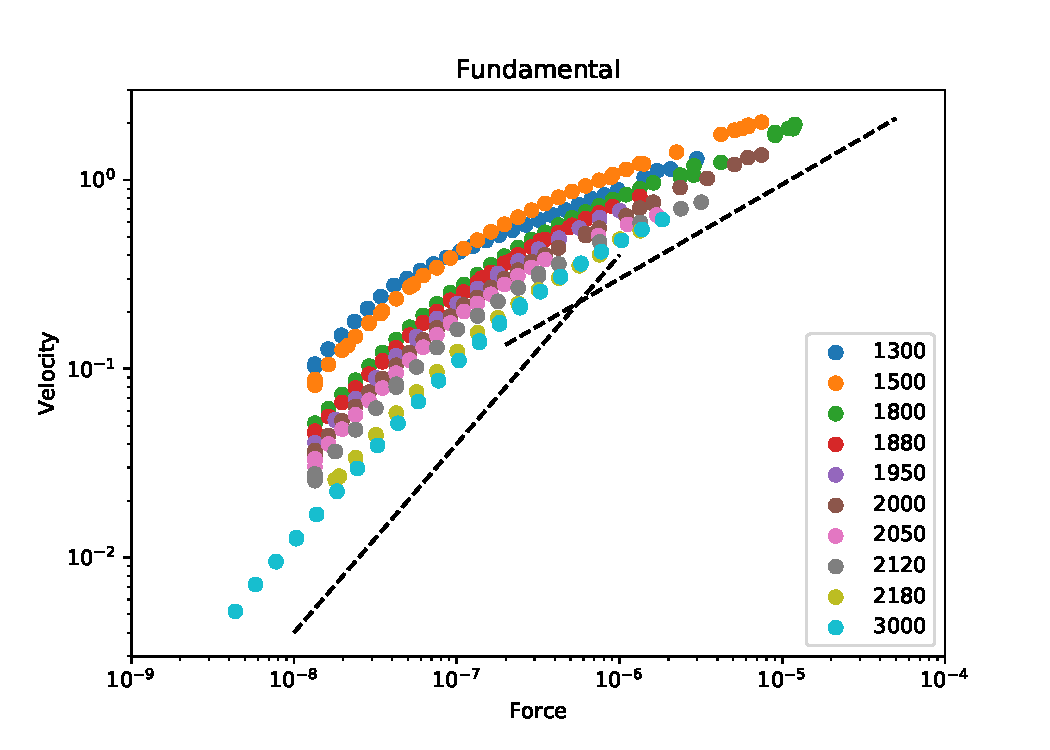
\includegraphics[width=0.8\textwidth]{graphics/results/fund-force_vel}
% 	\caption{Velocity against force}
% 	\label{fund_vel_force}
% \end{figure}
%
% Overtone:
%
% \begin{figure}[h]
% 	\centering
% 	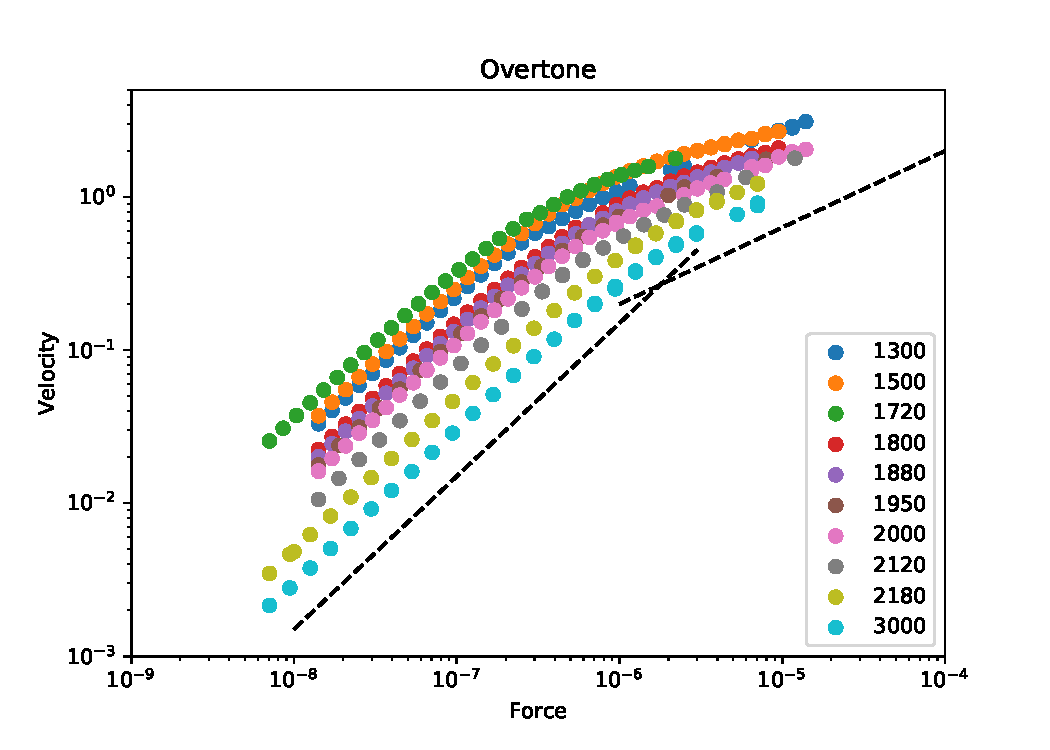
\includegraphics[width=0.8\textwidth]{graphics/results/over-force_vel}
% 	\caption{Velocity against force}
% 	\label{over_vel_force}
% \end{figure}
%
% Fundamental drag coefficient:
%
% \begin{figure}[h]
% 	\centering
% 	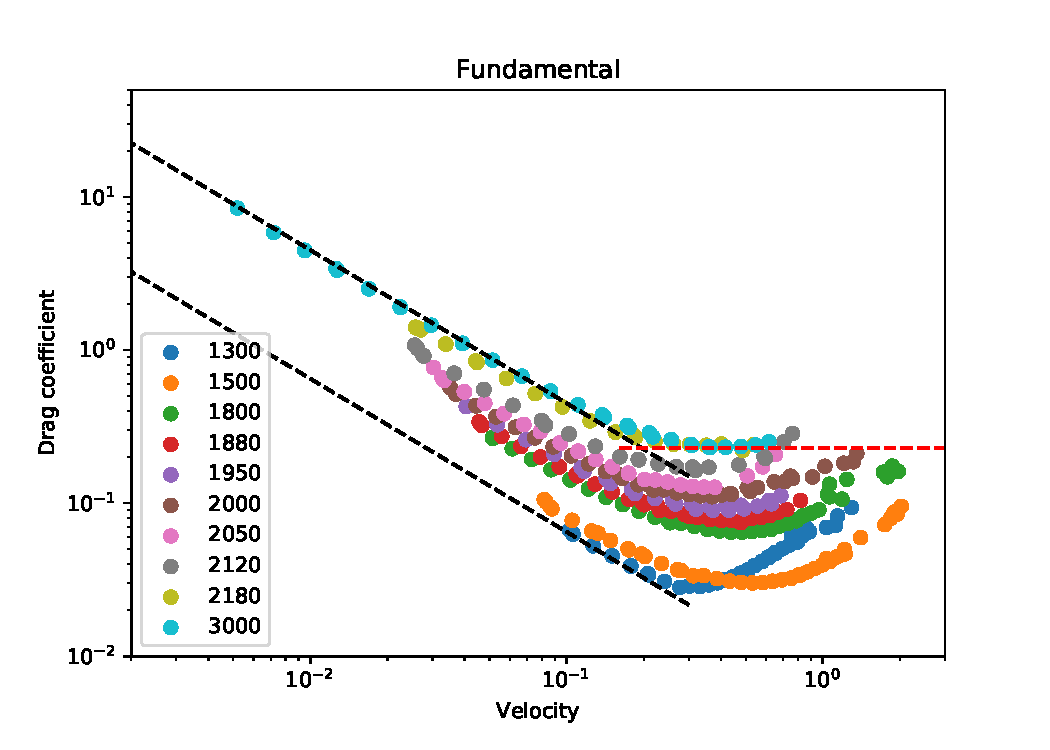
\includegraphics[width=0.8\textwidth]{graphics/results/fund-coeff_vel}
% 	\caption{Drag coeff against velocity}
% 	\label{fund_drag_vel}
% \end{figure}
%
% Overtone drag coefficient:
%
% \begin{figure}[h]
% 	\centering
% 	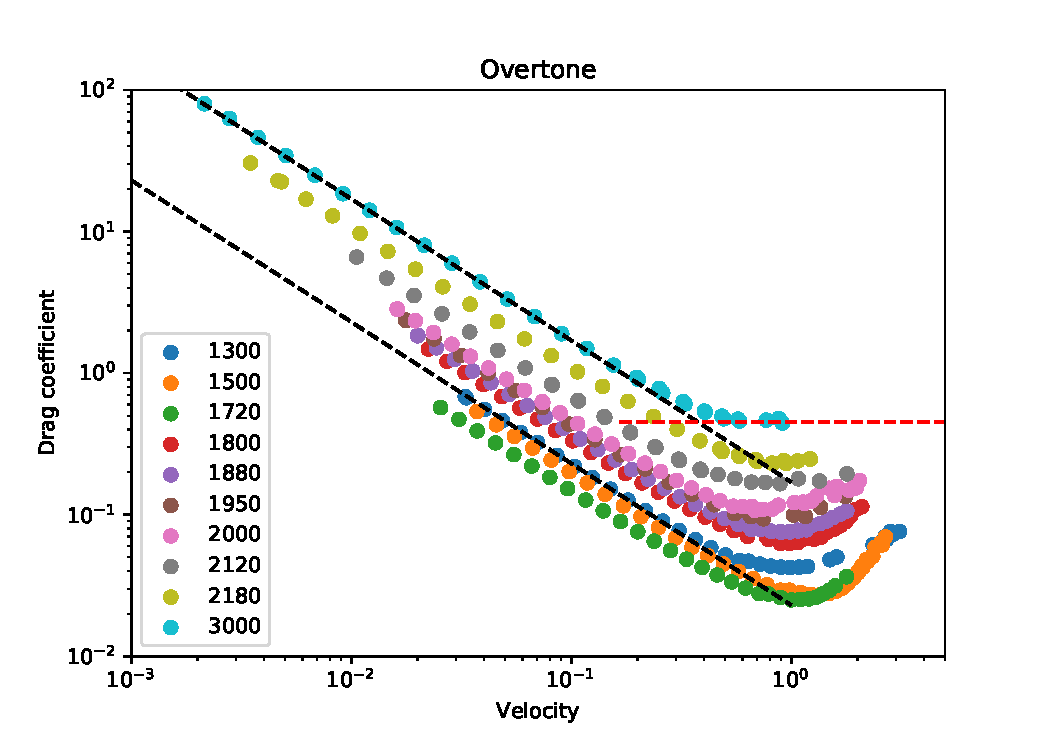
\includegraphics[width=0.8\textwidth]{graphics/results/over-coeff_vel}
% 	\caption{Drag coeff against velocity}
% 	\label{fund_drag_vel}
% \end{figure}
%
%
%
% Fundamental Donnelly:
%
% \begin{figure}[h]
% 	\centering
% 	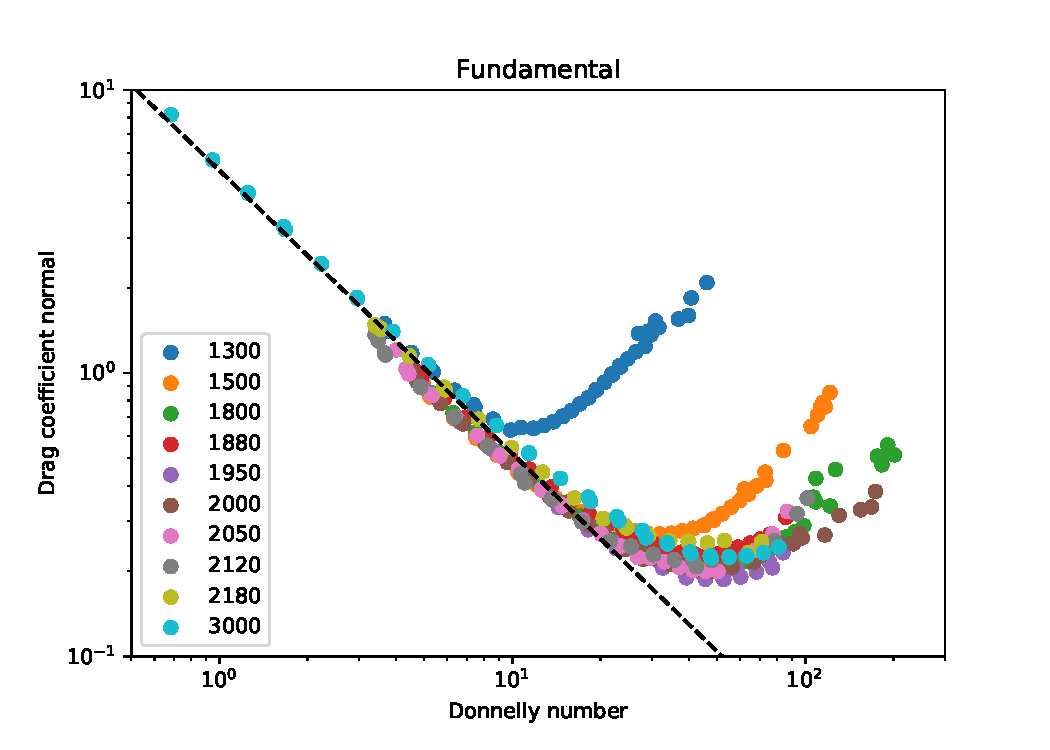
\includegraphics[width=0.8\textwidth]{graphics/results/fund-donnelly}
% 	\caption{Donnelly num against velocity}
% 	\label{fund_donnelly}
% \end{figure}
%
% Overtone Donnelly:
%
% \begin{figure}[h]
% 	\centering
% 	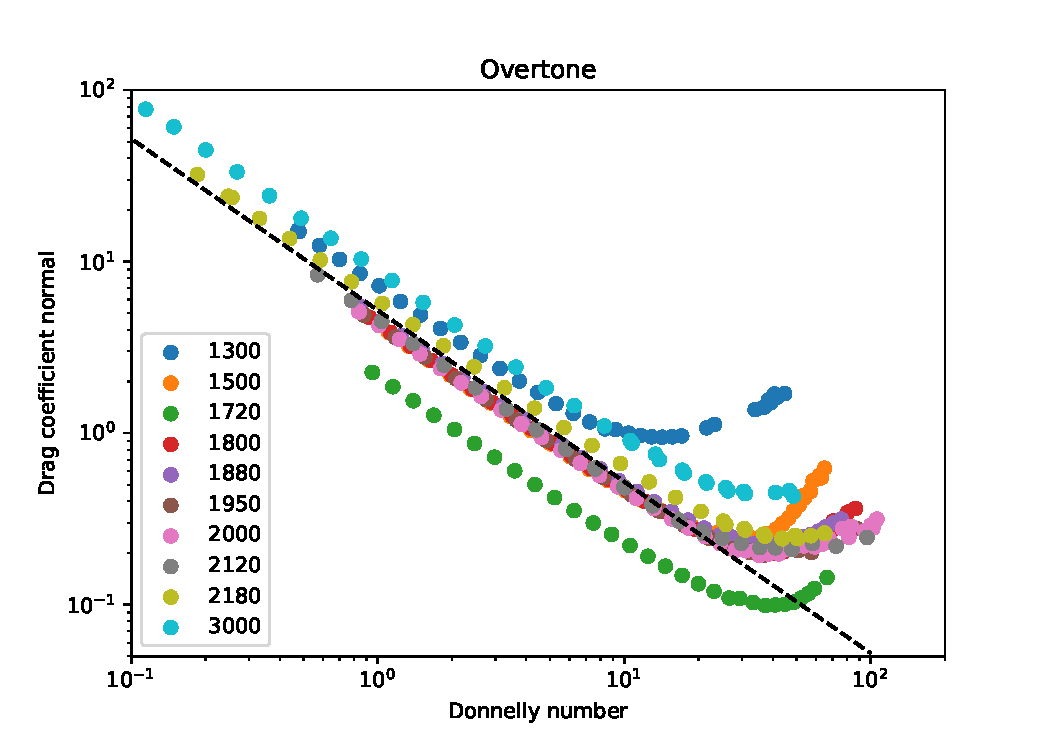
\includegraphics[width=0.8\textwidth]{graphics/results/over-donnelly}
% 	\caption{Donnelly num against velocity}
% 	\label{over_donnelly}
% \end{figure}
%
%
%
% Fundamental phase diagram:
%
% \begin{figure}[h]
% 	\centering
% 	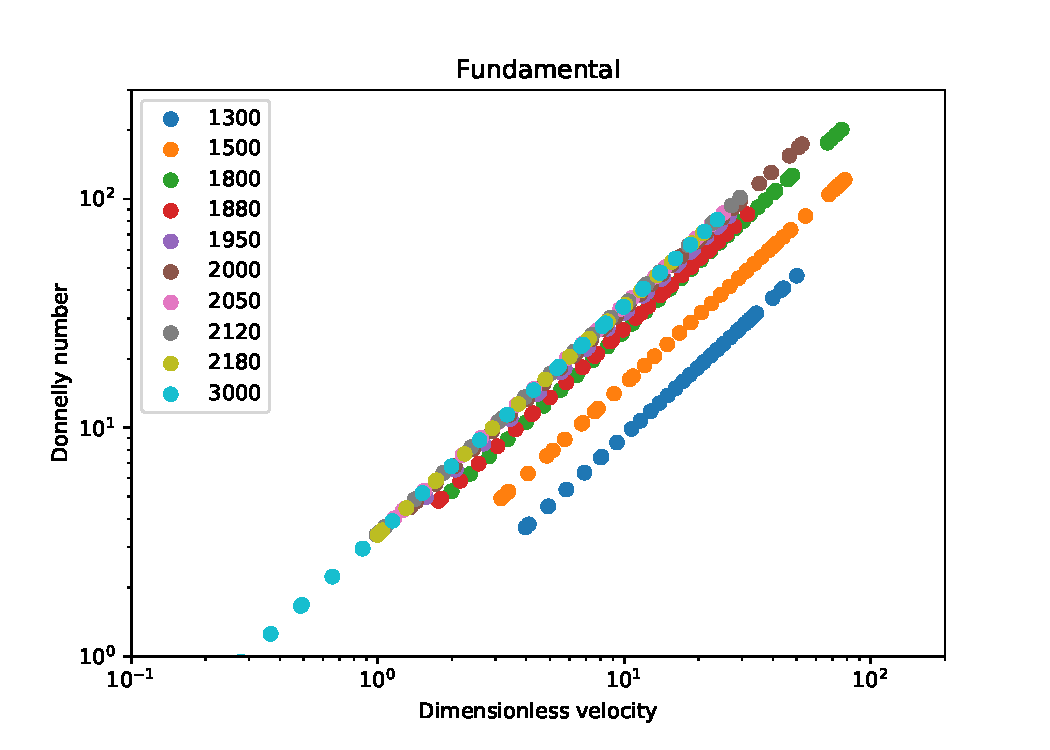
\includegraphics[width=0.8\textwidth]{graphics/results/fund-phase}
% 	\caption{Donnelly num against dimless velocity}
% 	\label{fund_phase}
% \end{figure}
%
% Overtone phase diagram:
%
% \begin{figure}[h]
% 	\centering
% 	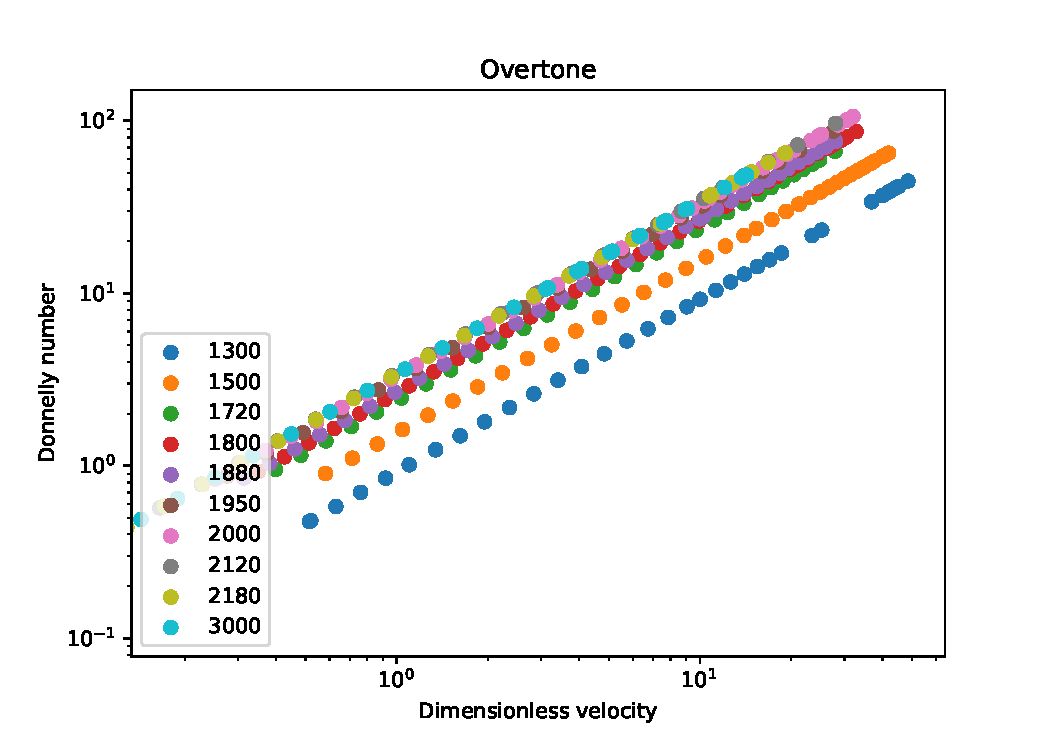
\includegraphics[width=0.8\textwidth]{graphics/results/over-phase}
% 	\caption{Donnelly num against dimless velocity}
% 	\label{over_phase}
% \end{figure}
%
%
% \newpage
